\documentclass[a4paper]{article}

%%% Encodage, langues, guillemets, ... %%%
%\usepackage[french]{babel}       
\usepackage[utf8]{inputenc}
%\usepackage{aeguill}
%\usepackage{fullpages}
%\usepackage{glosstex}
%\usepackage{setspace}

\usepackage{listings}
\usepackage{lscape}

%%% Inclusion images et feuilles pdf %%%
\usepackage{graphicx}
\usepackage{pdfpages}
%\usepackage{wrapfig}
\usepackage{geometry}

%%% Inclusion url et liens %%%
\usepackage{hyperref}
\usepackage{url}

% Inclure texte brut sans formattage
%\usepackage{moreverb}
% Changement des puces de enumerate
\usepackage{enumerate}

%%% Symboles, Math�matique %%%
% Math�matiques
\usepackage{amsmath}
\usepackage{amssymb}

%%% Sch�mas
% Graphes, g�om�trie et autres
\usepackage{tikz}
% Circuts �lectriques
%\usepackage{circuitikz}

\newcommand{\ns}[0] {{\em ns}}

\begin{document}
\large

%guardpage.tex

\setlength{\parskip}{5mm plus2mm minus2mm}
\lstset{language=tcl, showstringspaces=false, numbers=left, numberstyle=\tiny, tabsize=4}
 
{\setlength{\parindent}{0cm}
AbdelMourhit MAZIANE \\
Swan ROCHER
}
\vfill
{\centering \Huge \bfseries Simulation de r\'eseaux IP avec \ns \par}
\vfill
2012 \hfill Universit\'e Montpellier 2
\newpage
\tableofcontents
\thispagestyle{empty}
\pagenumbering{arabic}
\newpage



%tp1_intro.tex

\section{Introduction}
Il est souvent difficile et long d'effectuer r\'ellement des tests de r\'eseaux, c'est
pourquoi il est pr\'ef\'erable d'utiliser des outils de simulation.
Ici, nous nous int\'eressons au logiciel \ns, et nous \'etudions les d\'ebits moyens,
taux de perte de paquets ainsi que la taille de la file d'attente.
Le but de ce TP \'etant de nous familiariser avec cet outil, les diff\'erents tests
effectu\'es sont tr\`es simples et ont un int\^eret pratique discutable.



%tp1_topo.tex

\section{Topologie du R\'eseau}

Le r\'eseau simul\'e est compos\'e de deux sites avec un lien du premier vers le second
d'une capacit\'e de 2Mb/s et de latence 20ms.
Sa file d'attente de type {\em DropTail} peut supporter 100 paquets.

Quatre trafics sont mis en place :
\begin{itemize}
	\item la premi\`ere connexion suit le protocole UDP, son d\'ebit est exponentiel, la
	dur\'ee moyenne des p\'eriodes d'activit\'e est de 10ms, tandis que celles
	d'inactivit\'e durent 5 ms ;
	\item les trois autres suivent un protocole TCP, et sont de d\'ebits constants, leurs
	latences respectives sont de 50ms, 100ms et 150ms.
\end{itemize}

Le débit moyen théorique de chacune de ces connexions est de 1Mb/s, il était donc
nécessaire de calculer le débit crête du lien UDP de manière à pouvoir obtenir un débit
moyen théorique juste malgré les périodes d'inactivité.\\
$\bar{\lambda} = \frac{\lambda_{crete} \times ON}{ON + OFF}$\\
On a donc : $\lambda_{crete} = \frac{(ON + OFF) \times \bar{\lambda}}{ON}$.\\
On en déduit $\lambda_{crete} = 1.5 Mb/s$.

De plus il fallait également calculer la taille des paquets des connexions TCP de manière
à assurer le débit moyen théorique de 1Mb/s.\\
$\bar{\lambda} = \frac{taille_paquet}{intervalle}$\\
On a donc : $taille_paquet = \bar{\lambda} \times intervalle$.\\
Les tailles de paquets sont donc respectivement :
\begin{itemize}
	\item 6250 octets,
	\item 12500 octets,
	\item 18750 octets.
\end{itemize}

Les quatre connexions sont lancées simultanément au démarrage, et sont stoppées à 10
secondes du démarrage.

\hbox{
	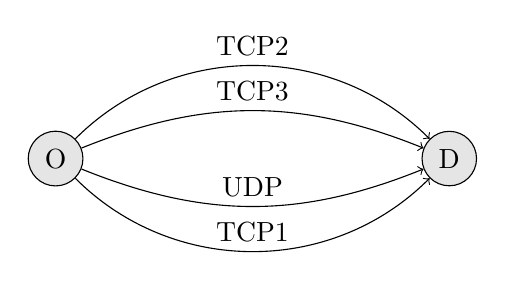
\begin{tikzpicture}
		\node[circle,draw,fill=black!10] (O) at (0,0) {O};
		\node[circle,draw,fill=black!10] (D) at (5,0) {D}
			edge[<-,bend left=22] node[above] {UDP} (O)
			edge[<-,bend left=45] node[above] {TCP1} (O)
			edge[<-,bend right=45] node[above] {TCP2} (O)
			edge[<-,bend right=22] node[above] {TCP3} (O)
			;
	\end{tikzpicture}
%\caption{Topologie}
\label{topo_fig}
}


%tp1_source.tex

\section{Code Source}
\lstinputlisting{../src/tp1.tcl}


%tp1_result.tex

\section{R\'esultats}


\input{tp1_conclusion.tex}

%\input{tp2_intro.tex}
%\input{tp2_topo.tex}
%\input{tp2_source.tex}
%\input{tp2_result.tex}

\end{document}

